\chapter{Kliens oldali technológiák}\label{ch:kliens}

\begin{osszefoglal}Az alkalmazás kliens oldali része egy single-page application (egyoldalas alkalmazás) \cite{SPA}, amelynek fejlesztése az AngularJS keretrendszer segítségével történt. A keretrendszer és az UI-Router által biztosított direktívák teszik lehetővé az alkalmazás különböző nézeteinek dinamikus felépítését, illetve a nézetek közötti egyszerű váltást, navigálást. A különböző nézetek elrendezése és megjelenítése az \texttt{index.html}-en, valamint a responsive design kialakitása a Bootstrap keretrendszer segítségével történik \cite{Bootstrap}.
\end{osszefoglal}

\section{Kliens oldali architekturális megoldások}
Az E-migrated alkalmazás kliens oldali MVC-t (Model-View-Controller) alkalmaz \cite{WebMVC}, ezáltal elkülönítve a nézetet az adatoktól és a vezérléstől. A kliens oldali MVC esetében a szerver csak statikus erőforrásként szolgál, nem teljesen felépített nézeteket küld vissza, csupán az ezek rendereléséhez szükséges adatokat szolgáltatja REST erőforrások formájában. A kliens oldal felelős ezek feldolgozásáért és megfelelő megjelenítéséért a kapott adatok és a meglévő sablonok alapján.
Az alkalmazás kliens oldalának architekturális megoldásai \aref{fig:ClientArchitecture} ábrán lathatóak. 

\begin{figure}
  \centering
  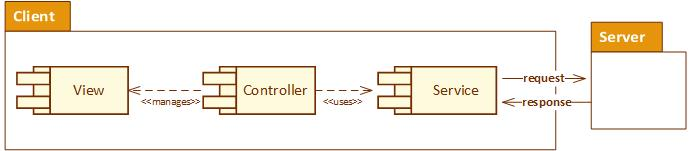
\includegraphics[width=0.9\linewidth]{images/ClientArchitecture}
  \caption{Az alkalmazás megjelenítési rétegét a kliens oldali komponens képviseli, a \textit{View}, \textit{Controller} és \textit{Service} modulok által. }
  \label{fig:ClientArchitecture}
\end{figure}

A \texttt{View} réteg biztosítja az alkalmazás felhasználói felületének megjelenítését. A felhasználók ezzel a réteggel lépnek direkt kapcsolatba, mely interakciókat a \texttt{Controller} észleli és irányítja. A \texttt{Controller} továbbítja a klienstől érkező kéréseket a service-eknek és a tőlük érkező válaszok alapján frissíti a nézetet. A \texttt{Service} réteg kommunikál a szerver API rétegével, JSON formátumú aszinkron kéréseket küldve és a válasz érkezése után továbbítja azokat a kontrollereknek. 

A webes komponens struktúrája az átláthatóság és az egyszerű bővíthetőség érdekében több, egymástól elkülönített részből épül fel, melyek a következők: \textit{services}, \textit{controllers}, \textit{directives} és \textit{config}. Az első kettő értelemszerűen a \texttt{Service} és a \texttt{Controller} rétegeket foglalja magába, míg a \textit{directives} modul tartalmazza a csapat által megírt direktívákat, amelyek hozzájárulnak a bonyolult nézetek egyszerűbb kezeléséhez és megjelenítéséhez. A \textit{config} modulban találhatóak a különböző konfigurációs beállítások, többek között itt történik a kontrollerek nézetekhez való hozzárendelése. 

\section{AngularJS}
\label{sec:angularjs}
Az AngularJS egy olyan JavaScript alapú, nyílt forráskódú keretrendszer, amely lehetővé teszi a kliens oldali MVC megvalósítását, illetve single-page alkalmazások egyszerű fejlesztését. Kiegészíti a HTML nyelvet különböző direktívákkal, így biztosítva a dinamikus nézetek létrehozását és a kétoldali adatkötést (two way data binding) \cite{AngularJS}.

A kétoldali adatkötés teszi lehetővé a nézetek automatikus frissítését, amennyiben a hozzárendelt modell objektum értéke változik, illetve a modell frissítését, ha a nézeten történik változás, ezáltal megszabadítva a fejlesztőket a DOM elemek kezelésétől és az ehhez tartozó kódok implementálásától. Az AngularJS modell objektumai egyszerű JavaScript objektumok.

A keretrendszer által biztosított Dependency Injection minta lehetővé teszi a komponensek számára a külső függőségeik használatát anélkül, hogy ismerniük kellene  a háttérben levő implementációt, ezáltal tesztelhetőbbé és átláthatóbbá téve a kódot. A keretrendszer injektálja és példányosítja is az adott függőséget, így nincs szükség bonyolult konstruktorhívásra.     

A DOM elemek viselkedésének meghatározása kontrollerek segítségével történik, ezáltal elválasztva a nézetet a vezérléstől, és így átláthatóbb, könnyebben tesztelhető alkalmazás-struktúrát hozva létre. A kontroller felelős a kliens interakcióinak figyeléséért és az ezekre való megfelelő viselkedés aktiválásáért. 



A keretrendszer lehetőséget nyújt új direktívák deklarálására is, amelyek segítségével alkalmazás specifikus, újrafelhasználható DOM elemek vezethetőek be a HTML nyelvbe. 


\section{Web Controller}
\label{sec:webController}
A Web Controller a kliens oldali MVC üzleti logika részét képezi. Felelős a nézetek inicializásáért, azok frissítéséért, illetve a service rétegektől érkező adatok megfelelő megjelenítéséért. 

Minden nézethez hozzárendelhető egy vagy több vezérlő, amelyeket az \texttt{ng-controller} direktívák segítségével vagy az \texttt{app.config} állományban állíthatunk be. A kontroller létrejövetelekor hozzárendelődik a DOM-hoz és egy \texttt{\$scope} objektumon keresztül hozzáférést kap a nézet elemeihez, amelyeket ezáltal irányíthat és módosíthatja tulajdonságaikat. 

A nézet inicializálása az \texttt{ng-init} direktívának megadott metódus aktiválása által történik, automatikusan. Minden a nézetben használni kívánt metódust hozzá kell rendelni a vezérlő \texttt{\$scope}  objektumához. Ez teszi lehetővé, hogy a kontroller különböző események hatására megfelelő viselkedést biztosíthasson. Ilyen esemény lehet például egy gombra való kattintás, amely során a gomb \texttt{ng-click} direktívájának értékeként megadott metódus aktiválódik. \Aref{lst:ngClick} kódrészletben látható a meghívó kérések kilistázása, amelyeket az adminisztrátor elfogadhat, elutasíthat vagy törölhet, kattintása során aktiválva a \texttt{RequestInvitation} kontroller megfelelő metódusát.

\begin{listing}
  \inputminted[fontsize=\small]{html}{progfiles/ngClick.html}
  \caption{Meghívó kérések kilistázása az adminisztrátor számára\protect{,} amelyeket elfogadhat\protect{,} elutasíthat vagy törölhet. Rákattintva a megfelelő gombra akitválja az \texttt{ng-click} direktíva értékeként megadott\protect{,} a \texttt{RequestInvitation} kontrollerhez tartozó metódusok valamelyikét.}
  \label{lst:ngClick}
\end{listing}

Mivel a kontroller továbbítja a kéréseket a service réteg számára, amely aszinkron hívásokon keresztül kommunikál a szerverrel, ezért a válasz is aszinkronon érkezik meg, így nem tudjuk garantálni a megfelelő betöltési sorrendet. Annak érdekében, hogy ne jelenjenek meg az oldalon félkész adatok, minden kontroller rendelkezik egy \texttt{loaded} attribútummal, amely kezdetben hamis és csak akkor vált értéket, és teszi láthatóvá a nézet adott részét, ha a kontroller minden szükséges adatot megkapott a service rétegtől. Az oldal bizonyos részének elrejtését az  \texttt{ng-show} és az \texttt{ng-if} direktívák teszik lehetővé. 

A Web Controller komponens kommunikál a Web Service-szel a szervertől szükséges adatok lekérése és megjelenítése érdekében, és részt vesz a kétirányú adatkötésben a különböző eseményeket kezelő függvények biztosítása és a nézetek adatainak megfelelő vezérlése által. 

\section{Web Service}
\label{sec:webService}
A Web Service réteg kommunikál az alkalmazás szerverével, HTTP protokollon keresztül, a REST konvencióknak megfelelő API hívások által. 

A service-ek különböző metódusokat publikálhatnak, amelyeket a kontrollerek elérhetnek, ha injektálják az adott szolgáltatást. A web service a kontrollertől érkező adatok alapján felépíti a szerver számára a megfelelő kérést és egy \texttt{\$http} objektum segítségével elküldi azt (\ref{lst:httpKeres}. kódrészlet).

\begin{listing}
  \inputminted[fontsize=\small]{js}{progfiles/httpKeres.js}
  \caption{A \texttt{suspendUserService} által küldött aszinkron kérés egy \texttt{\$http} objektum segítségével.}
  \label{lst:httpKeres}
\end{listing}
A szervertől érkező válaszokat \texttt{promise} objektumok formájában küldik vissza a kontroller részére, a \texttt{resolve} illetve a \texttt{reject} metódusok által jelezve, hogy lépett-e fel hiba a kérés teljesítése során vagy sem. 

A szerverhez küldött aszinkron kérések csökkentése érdekében a service osztályok tárolhatnak különböző adatokat, melyeket a kontrollerek getter és setter metódusok segítségével érhetnek el. Ezeket az adatokat az E-migrated alkalmazás a \texttt{\$localStorage} objektum segítségével tárolja. Annak érdekében, hogy a tárolt adatok mindig naprakészek maradjanak, az adott értéket módosító setter metódus hívásakor, a servicek nem csak a szerver irányába küldik el a kérést, hanem frisítik a \textit{LocalStorage}-ban levő értéket is. Ezáltal nem szükséges a kontrollertől érkező kérések mindenikét tovább irányítani a szerver fele, elég ha a service lekéri az adatokat a  \textit{LocalStorage}-ból. Ezt a mechanizmust lehet használni az alkalmazás ideiglenes offline működésének biztosítására is. 

\section{Angular UI-Router}
\label{UI-Router}

Az Angular-UI Router egy kliens oldali keretrendszer, amelyet AngularJS-ben írt single-page alkalmazások számára fejlesztettek ki \cite{uirouter}. A UI-Router rendelkezik az AngularJS beépített \texttt{ng-router}-ének minden funkcionalitásával, viszont van két nagy előnye: a többszörös nézet, illetve a beépített nézet. 

A legtöbb webes alkalmazás rendelkezik  fejéccel, fő tartalommal, lábjegyzettel, illetve bizonyos esetekben egy oldalmenüvel. Az AngularJS alapértelmezett router-jével szemben, a UI-Router megengedi több nézet elhelyezését egy HTML oldalon belül, melyek közül mindegyik külön névvel, illetve külön kontrollerrel rendelkezhet. Ennek előnye, hogy ezek a nézetek újra felhasználhatóak, az alkalmazás átláthatóbb és könnyebben bővíthető. 

Beépített nézet használható olyankor, amikor egymáshoz szorosan kapcsolodó nézeteket szeretnénk ugyanazon oldalon megjeleníteni. Például bal oldalon megjelenik egy felsorolás és ezen felsorolás elemeire kattintva, jobb oldalon megjelenik egy űrlap, ahol szerkeszthetjük, módosíthatjuk az elemeket.

\begin{listing}
  \inputminted[fontsize=\small]{js}{progfiles/app.conf.js}
  \caption{A fő tartalmat megjelenítő ui-view-ba a külöböző állapotok dinamikus behelyettesítése a UI-Router segítségével történik. Az állapot-nézet megfeleltetések az \texttt{app.conf.js} állományban a \texttt{\$stateProvider.state()} függvény segítségével valósulnak meg.  Például a \texttt{'home'} állapothoz hozzárendeli a \texttt{'/home'} URL-t, és a \texttt{'google-map.html'} sablont, hozzárendeli a \texttt{GoogleMapController}-t és beállítja a megfelelő jogosultságokat. Amennyiben egy felhasználó nem rendelkezik a megfelelő jogosultsággal a \texttt{\$urlRouterProvider.otherwise('/home')} függvény aktiválódik és vissza lesz térítve a főoldalra. }
  \label{lst:appconf}
\end{listing}



Az E-migrated alkalmázás kliens oldalán az \texttt{index.html} tartalmaz két \texttt{ui-view} direktívát, az első a fejlécben található menü, a második pedig maga a fő tartalom. A fő tartalom \texttt{ui-view}-jának neve \texttt{mainContainer} és ez lesz majd helyettesítve dinamikusan, a UI-Router által, a különböző állapotokkal. 


Az \textit{állapot} és \textit{nézet} közti megfeleltetés az \texttt{app.conf.js} állományban történik, ahol a \texttt{\$stateProvider state()} függvényének segítségével, minden állapothoz hozzárendelődik egy template URL, egy effektív URL és bizonyos esetekben egy kontroller is, valamint itt van beállítva, hogy melyik nézetet milyen jogosultsággal rendelkező felhasználó jeleníthet meg (\ref{lst:appconf}. kódrészlet). Amennyiben egy felhasználó nem rendelkezik a megfelelő jogosultsággal az \texttt{\$urlRouterProvider} \texttt{.otherwise('/home')} függvény aktiválódik és vissza lesz térítve a főoldalra. A szerver oldali ellenőrzés miatt, nem férhetnének hozzá a felhasználók érzékeny adatokhoz, viszont a kliens oldali ellenőrzés előnye, hogy már a UI-Router el tudja dönteni, hogy van-e jogosultsága egy adott felhasználónak megtekinteni egy nézetet, így a kérés szerver oldalra való továbbítása nélkül visszatérít a főoldalra.

Az alkalmazásban beépített nézeteket alkalmaz a profil szerkeztése nézet (\ref{fig:fiok_torlese}. ábra), valamint az bejegyzéseket megjelenító oldal is (\ref{fig:osszes_bejegyzes}. ábra).

A felhasználói profil szerkesztése esetében van egy fő view, az \texttt{edit-profile.html} amelyhez az \texttt{editProfile} státusz van hozzárendelve és amely tartalmaz egy baloldali menüsort, illetve a menü elemeinek szerkesztésére alkalmas nézetet. Ebben a \texttt{ui-view} direktívában lesznek megjelenítve az \texttt{editProfile} alstátuszai pl. az \texttt{editProfile.changeGeneralData} állapot. A leszármazott állapotok rendelkezhetnek külön kontrollerrel, de öröklik az ősállapot kontrollerét, így használhatják annak függvényeit is. Ebben az esetben a leszármazott állapotok mind az \texttt{EditProfileController}-t használják. 




\section{Google Map integráció}
\label{sec:googleMap}


Az Angular Google Maps teszi lehetővé az alkalmazás főoldalát betöltő lényeges komponens, a szakembereket csoportosító világtérkép megjelenítését. Ez a könyvtár olyan direktívák összessége, amelyek lehetővé teszik a Google Maps beintegrálását AngularJS alkalmazásokba, anélkül, hogy ismerni kellene a Google Maps API részleteit, és olyan jól ismert Google Maps objektumokat biztosítanak, mint például markerek, ablakok, vonalak a térképen stb. \cite{AngularGoogleMap}

A Google Maps könyvtár által biztosított térképjelzők testreszabhatóak, illetve egy \texttt{MarkerClusterer} objektum segítségével csoportosíthatóak a térképen (\ref{lst:markerClusterer}. kódrészlet). A jelzőkhöz különböző figyelők rendelhetőek, amelyek adott események hatására aktiválódnak, ilyen például a térképre való közelítés illetve a térképjelzőkre való kattintás. Közelítéskor a régiók lebomlanak kisebb területekre, részletesebben mutatva a szakemberek eloszlását. 
\begin{listing}
  \inputminted[fontsize=\small]{java}{progfiles/MarkerClusterer.js}
  \caption{A Google Maps könyvtár által biztosított térképjelzők testreszabhatóak, illetve egy \texttt{MarkerClusterer} objektum segítségével csoportosíthatóak a térképen.}
  \label{lst:markerClusterer}
\end{listing}

Az E-migrated alkalmazás kibővíti a Google Maps könyvtár \texttt{googleMap} direktíváját egy új, alkalmazás specifikus direktívával. Ez gondoskodik a térképjelzők létrehozásáról és koordináták szerinti elhelyezéséről a térképen, valamint a felhasználói információk megfelelő megjelenítéséről a jelzőkre kattintva. Ha egy adott régióban többen laknak, mint három, a felhasználói adatok nem az alapértelmezett, térképen felugró ablakokban jelennek meg, hanem a térkép mellett egy jobboldali panelben. 





 